\documentclass{statsoc}
\usepackage[left=7mm,right=15mm]{geometry} % required for statsoc+pdflatex
\usepackage{vmargin} % required for statsoc+pdflatex

%\usepackage{amsthm} %not compatible with statsoc
\usepackage{amsmath,amssymb,hyperref}
%\usepackage{esint}
\usepackage{natbib}
\usepackage{color}
\usepackage{pdfsync}
\usepackage{float}
\usepackage{graphicx}
\usepackage{subfigure}
\usepackage{xspace}


%\makeatletter
%%%%%%%%%%%%%%%%%%%%%%%%%%%%%% Textclass specific LaTeX commands.
% \theoremstyle{plain}
 \newtheorem{thm}{Theorem}
%   \theoremstyle{plain}
   \newtheorem{lem}[thm]{Proposition}

%%%%%%%%%%%%%%%%%%%%%%%%%%%%%% User specified LaTeX commands.
\newcommand{\eqdef}{\stackrel{\Delta}{=}} % not used
\newcommand{\x}{\mathbf{x}}
\newcommand{\h}{\mathbf{h}}
\newcommand{\myprod}{\prod_{\substack{i=1\\i\neq \h_t^n(s)}}^{N_x}}
\newcommand{\myprodone}{\prod_{\substack{i=1\\i\neq \h_t^n(1)}}^{N_x}}
\def\O{\mathcal{O}}
\newcommand{\SMCSQ}{SMC$^2$\xspace}
\newcommand{\col}[2]{{\color{#1}#2}}
\newcommand{\E}{\mathbb{E}} % Expectation
\newcommand{\iid}{\stackrel{iid}{\sim}}


%\usepackage{verbatim}
% comment/uncomment to show/hide comments in red
% hide:
%\newcommand{\brc}{\begin{comment}}\newcommand{\erc}{\end{comment}}
% show 
\newcommand{\brc}{\color{red}}\newcommand{\erc}{\color{black}}

% NC: THIS DOES NOT WORK, STRANGE BUG WITH \begin|end{comment}
% SO I COMMENTED ALL THE BLOCKS, search ``\brc'' to uncomment them

%\makeatother

%\usepackage{babel}
%\addto\extrasfrench{\providecommand{\og}{\leavevmode\flqq~}\providecommand{\fg}
%{\ifdim\lastskip>\z@\unskip\fi~\frqq}}



\title[\SMCSQ]{\SMCSQ: an efficient algorithm for  sequential analysis of state-space models}

\author[Chopin et al.]{N. CHOPIN}
\address{CREST-ENSAE}
\email{nicolas.chopin@ensae.fr}
\author[Chopin et al.]{P.E. JACOB}
\address{CREST \& Universit\'e Paris Dauphine}
\email{pierre.jacob@ensae.fr}
\author[Chopin et al.]{O. PAPASPILIOPOULOS}
\address{Universitat Pompeu Fabra}
\email{omiros.papaspiliopoulos@upf.edu}

\begin{document}


\section{Numerical illustrations}\label{sec:numerics}


An initial study which illustrates \SMCSQ in a range of examples 
of moderate difficulty is available from the second author's web-page as supplementary 
material,see 
\href{http://sites.google.com/site/pierrejacob/}{http://sites.google.com/site/pierrejacob/}. 
In that study, \SMCSQ was shown to 
typically outperform competing algorithms, whether in sequential
scenarios (where datapoints are obtained sequentially)
or in batch scenarios (where the only distribution of interest
is $p(\theta,x_{1:T}|y_{1:T})$ for some fixed time horizon $T$). 
For instance, in the former case,  \SMCSQ was shown to provide  smaller Monte Carlo errors
than the SOPF at a given CPU cost. In the latter case, 
\SMCSQ was shown to compare favourably to an adaptive version of the marginal
PMCMC algorithm proposed by \citet{PetersHosackHayes}. 

In this paper, our objective instead is to take a hammer to \SMCSQ, 
that is, to evaluate its performance on models that are regarded
as particularly challenging, even for batch estimation purposes. 
In addition, we treat \SMCSQ as much as possible as a black box: 
the number $N_x$ of $x$-particles is augmented dynamically (using the exchange step, see
Section \ref{sub:exchange}), as explained
in Section \ref{sec:increase}; the move steps are calibrated using the current particles, as 
described at the end of Section \ref{sub:An-idealized-algorithm}, and so on.  
The only model-dependent inputs are (a) a procedure
for sampling from the Markov transition of the model, $f_\theta(x_{t+1}|x_t)$,  and 
(b) a procedure for pointwise evaluation the likelihood $g_\theta(y_t|x_t)$
\textcolor{red}{and (c) a prior distribution on the parameters}. 
This means that the proposal $q_{t,\theta}$ is set to the default
choice $f_\theta(x_{t+1}|x_t)$. This also means that we may even 
treat models such that the density  $f_\theta(x_{t+1}|x_t)$ cannot be 
computed, even if it may be sampled from; this is the case
in the first application we consider. 

A generic \SMCSQ software package written in Python and C by the second author is available at 
\href{http://code.google.com/p/py-smc2/}{http://code.google.com/p/py-smc2/}. 

\subsection{Sequential prediction of asset price volatility}

\SMCSQ  is particularly well suited to tackle several of the
challenges that arise in the probabilistic modelling of financial time
series: prediction is of central importance; risk management requires
that parameter and model uncertainty is properly reflected in
prediction; stylized empirical features suggest the need for
non-linear modelling; the length of typical time series is large when
modelling 
medium/low frequency data and vast when considering 
high frequency observations; there exist several competing models hence
it is desirable to have a flexible algorithmic framework which allows
an almost-automatic exploration of the model space; for several
interesting models it is easy to simulate the state process dynamics forward but
harder (or impossible) to compute the system transition density. 

We illustrate some of these possibilities in the context of prediction
of daily volatility of asset prices. There is a vast literature on
stochastic volatility (SV) models; we simply refer to the excellent
exposition in  \cite{bns:real} for references, perspectives and
second-order properties. The generic framework for daily
volatility is as 
follows. Let $s_t$ be the value of a given
financial asset (e.g a stock price or an exchange rate) on the $t$-th
day, and $y_t=10^{5/2} \, \log(s_t/s_{t-1})$ be the so-called log-returns (the
scaling is done for numerical convenience). 
Then, the SV model specifies a state-space model
with observation  equation: 
\begin{equation}
  \label{eq:sv-obs}
  y_t = \mu + \beta v_t + v_t^{1/2} \epsilon_t \,, t\geq 1
\end{equation}
where the $\epsilon_t$ is a sequence of independent errors which are
assumed to be standard Gaussian. The process $v_t$ is known as the actual
volatility and  it is treated as a stationary stochastic
process. This implies that log-returns are stationary with mixed Gaussian
marginal distribution. The coefficient $\beta$ has both a financial
interpretation (as a risk premium for excess volatility) and a statistical one. The case $\beta \neq 0$
implies skewness for the marginal distribution of log-returns, a feature 
commonly observed in stock prices.  For modelling volatility in stock
prices log-returns (as opposed to exchange rates) it is important to include an extra term to deal with
the  so-called leverage effect. We deal with this in the sequel. 

Whereas most SV models agree on the observation
equation, they differ widely in the specification of the dynamics of
the actual volatility. Here we consider the class of L\'evy driven SV
models which were introduced in \cite{bns:ou} and have been
intensively studied in the last decade from both the mathematical
finance and the statistical community. 

This family of models is specified via a  continuous-time model for the joint
evolution of log-price and spot (instantaneous)
volatility, which are driven by
Brownian motion and L\'evy process respectively. The actual volatility
is the integral of the spot volatility over daily intervals, and the
continuous-time model  translates into
a state-space model for $y_t$ and $v_t$ as we show below.   Details can be
found in Sections 2 (for the continuous-time specification) and 5
(for the state-space
representation) of the original article.
 Likelihood-based inference for this class of models is recognized
 as a very challenging problem, and it 
 has been
undertaken among others in \cite{robe:papa:dell:2004,grif:steel:ou}
and most recently in \cite{PMCMC} using PMCMC. On the other hand,
\cite{bns:real} develop quasi-likelihood methods using the Kalman filter based on an
approximate state-space formulation suggested by the second-order properties
of the $(y_t,v_t)$ process.  


The family of models is generated by varying  the
L\'evy process that drives the spot volatility. When this process is
expressed by means of an infinite 
rate Poisson process, the system transition density is typically
intractable and available  methods rely on
approximations for simulating the state process. In these cases, 
although it is also subject to approximation bias, PMCMC appears to
have a comparative advantage over alternative MCMC 
methods, see for example  Section 3.2 of \cite{PMCMC}.  
In this study we take instead a specification of the background
driving L\'evy process  in terms of a finite rate Poisson process and consider 
multi-factor specifications of such models which include
leverage. This choice allows the exact simulation of the actual
volatility process, and permits direct comparisons to  the numerical
results  in Sections 4 of \cite{robe:papa:dell:2004}, 3.2 of 
\cite{bns:real} and 6 of \cite{grif:steel:ou}. Additionally, this case
is representative  of a system which can be very easily simulated
forwards whereas computation of its transition density is considerably
involved (see \eqref{eq:ssf} below). 



The specification for the
one-factor model is as follows. We parametrize the latent process as in
\cite{bns:real} in terms of $(\xi,\omega^2,\lambda)$ where $\xi$ and $\omega^2$ are
the stationary mean and variance of the spot volatility process, and
$\lambda$ the exponential rate of decay of its 
autocorrelation function.  The second-order properties of $v_t$ can be
expressed as functions of these parameters,
see Section 2.2 of \cite{bns:real}. The
state dynamics for the actual volatility are as follows: 
\begin{equation}
  \label{eq:ssf}
  \begin{split}
     k  & \sim  \mathrm{Poi}\left( \lambda \xi^2/\omega^2 \right) \quad 
 c_{1:k}  \iid  \mathrm{U}(t,t+1) \quad 
e_{i:k}  \iid  \mathrm{Exp}\left(\xi/\omega^2 \right)  \\ 
  z_{t+1}  & =  e^{-\lambda} z_t + \sum_{j=1}^k  e^{-\lambda(t+1-c_j)}
  e_j \\
v_{t+1} & =  {\frac{1}{\lambda}} \left [ z_t - z_{t+1} + \sum_{j=1}^k e_j
\right ] \\
x_{t+1} & =  (v_{t+1},z_{t+1})' \, .
  \end{split}
\end{equation}
In this representation, $z_t$ is the discretely-sampled spot
volatility process, and the Markovian representation of the state
process involves the pair $(v_t,z_t)$. The random variables $(k,c_{1:k},e_{1:k})$ are generated
independently for each time period, and $1:k$ is understood as the
empty set when  $k=0$. These system dynamics imply a
$\Gamma(\xi^2/\omega^2,\xi/\omega^2)$ as stationary distribution for $z_t$. 
Therefore, we take this to be the initial distribution for $z_0$.


% *********************************************
% RESULTS: single factor, synthetic data

\subsubsection{Synthetic data set}

We simulate a synthetic data set of length $T = 1,000$, using 
$\mu = 0$, $\beta = 0$, $\xi = 0.5$, $\omega^2 = 0.0625$,
$\lambda = 0.01$; see top of Figure
\ref{fig:SVonefactor:observations}. These values were used also in the
simulation study of \cite{bns:real}. 
We launch $5$ independent runs using $N_\theta = 1,000$, a 
 ESS threshold set at $50\%$, and independent Hastings-Metropolis scheme
described in Section \ref{sub:An-idealized-algorithm}. The number $N_x$ is set to $100$, and 
increased whenever the acceptance rate goes below $20\%$; 
see bottom of Figure \ref{fig:SVonefactor:observations}.
Figure 
%\ref{fig:SVonefactor:overlaidKDEs}
\ref{fig:SVonefactor:Concentration} plots
the posterior marginal distribution of each parameter,
obtained at different times, and as estimated from the 
$5$ different runs. Monte Carlo variability across these runs 
seems very reasonable.  It is interesting to note that 
$N_x$ is systematically increased around time $400$, 
reacting to a large jump in the volatility. This is also reflected on
the posterior distributions of the parameters that determine the
volatility process, see  Figure
\ref{fig:SVonefactor:Concentration}. 
Note that SOPF, if run with $N=10^5$ particles,
collapses to one single particle at about $t=700$ and is thus
completely unusable in this context. 

\begin{figure}[H]
 \centering
 \subfigure[]{\includegraphics[width =
0.45\textwidth]{SVonefactor-observations}}
 \subfigure[]{\includegraphics[width =
0.45\textwidth]{SVonefactor-observations2}}
 \subfigure[]{\includegraphics[width = 0.45\textwidth]{SMC2acceptrates}}
 \subfigure[]{\label{fig:SVonefactor:increaseNx}\includegraphics[width = 0.45\textwidth]{SMC2increaseNx}}
 \caption{\label{fig:SVonefactor:observations} Single-factor stochastic volatility model, synthetic dataset.
Top row: observations (left) and squared observation (right) versus time. Bottom: Acceptance rate (left), number $N_x$
of $x-$particles (right) versus time obtained from $5$ repeated runs.
 }
\end{figure}


\begin{figure}[H]
 \centering
 \subfigure[]{\includegraphics[width =
0.90\textwidth]{SMC2theta1}}
 \subfigure[]{\includegraphics[width =
0.90\textwidth]{SMC2theta2}}
 \subfigure[]{\includegraphics[width =
0.90\textwidth]{SMC2theta3}}
 \subfigure[]{\includegraphics[width =
0.90\textwidth]{SMC2theta4}}
 \subfigure[]{\includegraphics[width =
0.90\textwidth]{SMC2theta5}}
 \caption{\label{fig:SVonefactor:Concentration} 
 Single-factor stochastic volatility model, synthetic dataset.
Overlaid kernel density estimators of the posterior distribution of the parameters,
at different times, $t=250,500,1000$, and  
computed from the particle samples obtained from $5$ repeated runs. 
The vertical dashed line indicates the true value, and solid red lines
the prior density. }
\end{figure}

\subsubsection{Extensive comparison with Liu \& West's particle filter}

We compare the results with Liu \& West's particle filter (referred to as L\&W in the following), where the hidden states are extended to include the parameters (as in SOPF), and where the $\theta$-components of the particles are diversified using a Gaussian move that leaves the variance of the particle sample unchanged (see REF TO L\&W). Compared to the general method described in
(REF TO L\&W), we do not implement any look-ahead scheme in the spirit of the auxiliary particle filter (REF TO APF), and hence
the proposal distribution for the $x$-components is set to $f_\theta(x_{t+1}\vert x_t)$. The $\theta$-components are updated using a Normal distribution as follows: at time $t+1$ the $\theta$-component of the $k$-th particle 
is drawn from $\mathcal{N}(\cdot \vert m^{(k)}_t, h^2 V_t)$, where the mean is $m^{(k)}_t = (1 - a) \theta_t^{(k)} + a \bar{\theta_t}$ with $a\in [0,1]$, ie an average between the particle and the empirical mean at the previous time, and the variance is defined by a product between
a smoothing parameter $h$ and the empirical variance $V_t$ at time $t$. By setting $a = \sqrt{1 - h^2}$, the
move step guarantees that the mean and the variance of the $\theta$-component remains constant. In the end the particles are indeed diversified, but the Gaussian move does not keep the distribution of the particles invariant:
it only guarantees the invariance of the first two moments, and the method is thus biased. We argue that this bias is significant for moderately long time series and therefore that exact method should be preferred.

Using again our $5$ runs of \SMCSQ on the synthetic data set, we look at their computing times in order to match the computational
effort of both methods. Consequently we decide to launch L\&W with $N = 200,000$ $(x,\theta)$-particles and we set the smoothing parameter $h$ to $10^{-1}$ (see below for the comparison between various values of $h$). The resulting computing times can be compared on Figure \ref{fig:SVonefactor:CT}. Unsurprisingly, L\&W 
runs are very consistent in terms of computing times, since the number of particles remains constant during each entire run and since the resample move steps, which occur at each iteration, all take the same time to complete. In comparison \SMCSQ shows a lot of variation in computing times, mainly because the number of $x$-particles does not reach the same value across the runs (see Figure \ref{fig:SVonefactor:increaseNx}) and also because the number of resample-move steps varies. The jumps on the right-hand side of Figure \ref{fig:SVonefactor:CT} correspond to resampling-move steps and to  increases of $N_x$. The figure shows that taking $N = 200,000$ allows a fair comparison between the methods.
Note also each of these runs took about or less than $7$ hours using a simple python script and only one processing unit of a 2008 desktop computer (equiped with an Intel Core 2 Duo E8400). Given that these methods could easily be parallelized, the computational cost can be greatly reduced; a $100\times$ speedup is plausible.
\begin{figure}[H]
  \centering
  \includegraphics[width = 0.7 \textwidth]{ComputingTime}
  \caption{\label{fig:SVonefactor:CT} Single-factor stochastic volatility model, synthetic dataset. Computing time (wall-clock) of $5$ independent runs of L\&W (left) and \SMCSQ (right) in seconds, against time.}
\end{figure}
Next we look at the posterior marginal distribution of each parameter obtained at time $t = 500$, which is about $100$ time steps after the large jump in volatility occuring at time $t = 407$. The results of both methods
are compared with a long PMCMC run with $N_x = 500$ $x$-particles and $N_i = 100,000$ iterations; $10,000$ iterations were discarded as burn-in. We used a Particle Marginal Metropolis--Hastings algorithm with a proposal
that is a mixture of a fixed gaussian random walk and a gaussian random walk using the already-generated chain to adapt its covariance matrix, following \cite{PetersHosackHayes}.
 The density plots are shown in Figure \ref{fig:SVonefactor:compareLW}.
\begin{figure}[H]
 \centering
%  \subfigure[]{\includegraphics[width =
% 0.90\textwidth]{MethodComparTheta1T500}}
%  \subfigure[]{\includegraphics[width =
% 0.90\textwidth]{MethodComparTheta2T500}}
  \includegraphics[width =\textwidth]{MethodComparTheta3T500}
%  \subfigure[]{\includegraphics[width =
% \textwidth]{MethodComparTheta3T500}}
%  \subfigure[]{\includegraphics[width =
% 0.90\textwidth]{MethodComparTheta4T500}}
%  \subfigure[]{\includegraphics[width =
% 0.90\textwidth]{MethodComparTheta5T500}}
 \caption{\label{fig:SVonefactor:compareLW} Single-factor stochastic volatility model, synthetic dataset.
Comparison between L\&W (left), \SMCSQ (middle) and a long PMCMC run (right) for the estimation of the posterior
marginal distribution of one out of the $5$ parameters.}
\end{figure}
The estimation of the marginal distribution of $\mu$ and $\beta$ gives similar results for all methods (not shown for brevity).
However, for $\xi$, $\omega^2$ and $\lambda$, \SMCSQ and PMCMC give similar results but L\&W results are significantly different (Figure \ref{fig:SVonefactor:compareLW} only shows the results for $\xi$, again for brevity). Closer inspection shows that the posterior distribution estimated using L\&W did not really react to the shock at time $t = 407$, compared to the other (exact) methods. Hence the bias of L\&W is obvious, even when the computational effort is matched. The choice of the smoothing parameter $h$ is not obvious and hence we try various values: $h_1 = 0.01$, $h_2 = 0.05$ and $h_3 = 0.1$.
The results for the same parameter $\xi$ are shown in Figure \ref{fig:SVonefactor:compareLWsmoothing} (again, a similar
discrepancy between L\&W and PMCMC was found for the parameters $\omega^2$ and $\lambda$).
We see that for the smallest value $h_1$, the variation between two runs becomes important, while
the bias is still large compared to the distribution estimated using PMCMC.
\begin{figure}[H]
 \centering
  \includegraphics[width =\textwidth]{CompareLWsmooth3T500}
%  \subfigure[]{\includegraphics[width =
% \textwidth]{CompareLWsmooth3T500}}
%  \subfigure[]{\includegraphics[width =
% 0.90\textwidth]{CompareLWsmooth4T500}}
%  \subfigure[]{\includegraphics[width =
% 0.90\textwidth]{CompareLWsmooth5T500}}
 \caption{\label{fig:SVonefactor:compareLWsmoothing} Single-factor stochastic volatility model, synthetic dataset.
Posterior distribution obtained using L\&W for one out of the $5$ parameters and for various values of $h$: $h_1 = 0.01$, $h_2 = 0.05$ and $h_3 = 0.1$. For each value of $h$, two independent runs are represented by overlaid estimated density curves.
The PMCMC posterior distribution is shown on the right for reference.}
\end{figure}

As expected, a biased representation of the posterior distribution can seriously damage the subsequent
statistical analysis. To illustrate this in the time series context, we look at the estimated log evidence
$\log p(y_{1:t})$, which is a building block for model choice. Figure \ref{fig:SVonefactor:evidence} shows the log evidence of each run, for each method, 
minus the ``reference log evidence'', taken as the mean of the log evidence of the $5$ \SMCSQ runs (since we know that \SMCSQ provides a consistent estimate).
We see that the log evidence estimated using L\&W is systematically biased, positively or negatively depending on the time steps, with a large discontinuity at time $t = 407$.
\begin{figure}[H]
  \centering
  \includegraphics[width = 0.9 \textwidth]{LogEvidenceVariationsAcrossRuns}
  \caption{\label{fig:SVonefactor:evidence} Single-factor stochastic volatility model, synthetic dataset.
Comparison between L\&W and \SMCSQ in terms of estimating the log evidence. The curves represent 
the estimated evidence of each run minus the reference log evidence, where the reference log evidence is the
mean across $5$ runs of the log evidence estimated using \SMCSQ .
}
\end{figure}

%****************************************************


\subsubsection{S\&P 500}

We now fit  L\'evy driven models of different complexity to
the S\&P 500 index. The data set 
is made of $753$ observations from January 3rd 2005 to December 31st
2007 and it is shown on Figure
\ref{subfig:SP500:observations2}. 

 \begin{figure}[H]
  \centering
  \subfigure[]{\label{subfig:SP500:increaseNx:multifactor}\includegraphics[
 width =
 0.45\textwidth]{SP500increaseNx}}
  \subfigure[]{\label{subfig:SP500:observations2}
 \includegraphics [ width =
 0.45\textwidth]{SP500observations2}}
  \subfigure[]{\label{subfig:SP500:acceptrates:multifactor}\includegraphics[width
 =
 0.45\textwidth]{SP500acceptrates}}
  \subfigure[]{\label{subfig:SP500:evidence}\includegraphics[width
 =
 0.45\textwidth]{SP500evidencecomparison}}
  \caption{\label{fig:SP500:observations} SP500 data. Top left: number $N_x$ of $x$-particles 
for the full model along the iterations over $3$
    independent runs. Bottom left: acceptance
    rates of the resample-move step for the full model over $3$
    independent runs. Top right: the S\&P 500 data from
    03/01/2005 to 21/12/2007 (squared values).  Bottom right:   log-evidence comparison between
    models (relative to the one-factor model). }
 \end{figure}

We first consider multifactor models. A multifactor model writes the
actual volatility as a sum of 
independent components each of which follows a L\'evy driven
model. These models have more flexibility to capture the dependence in
the log-returns, 
see for example Section 2.3 in \cite{bns:real}. Previous research
indicates that a two-factor model is sufficiently flexible, whereas
more factors do not add significantly when considering daily data, see
for example \cite{bns:real,grif:steel:ou} for L\'evy driven models and
\cite{chernov:multi} for diffusion-driven SV models.  We consider one
component which  describes long-term movements in the
volatility, with memory parameter $\lambda_1$, and another which
captures short-term variation,  with parameter 
$\lambda_2 >> \lambda_1$. The second component allows more freedom in
modelling the tails in the distribution of log-returns. The contribution of the slowly mixing
process to the overall mean and variance of the spot volatility is
controlled by the parameter $w \in (0,1)$. 
Thus, for this model
$x_t=(v_t,v_{1,t},z_{1,t},v_{2,t},z_{2,t})$ with
$v_t=v_{1,t}+v_{2,t}$, where each pair $(v_{i,t},z_{i,t})$ evolves
according to  \eqref{eq:ssf} with parameters $(w_i \xi,w_i 
\omega^2,\lambda_i)$ with $w_1=w, w_2=1-w$. The system errors are 
generated by independent sets of variables
$(k_i,c_{i,1:k},e_{i,1:k})$, and $z_{0,i}$ are initialized according
to the corresponding gamma distributions. 

Finally, we extend the observation equation to capture a significant
feature observed in returns on stocks: low returns provoke
increase in subsequent volatility, see for example \cite{black} for
an early reference. In parameter driven SV models, one generic
strategy to incorporate such feedback is to correlate the noise in the
observation and state processes, see \cite{harvey:shep}  in the
context of the logarithmic  SV model, and Section 3 of \cite{bns:ou}  for L\'evy
driven models.  We take up their suggestion, and re-write the
observation equation as 
\begin{equation}
  \label{eq:sv-obs-lev}
  y_t = \mu + \beta v_t + v_t^{1/2} \epsilon_t + \rho_1
  \sum_{j=1}^{k_1} e_{1,j} + \rho_2  \sum_{j=1}^{k_2} e_{2,j} -
\xi(w \rho_1  \lambda_1 + (1-w) \rho_2  \lambda_2) 
\end{equation}
where $e_{i,j}$ are the system error variables involved in the
generation of $v_t$ and $\rho_i$ are the leverage parameters which we
expect to be negative. Thus, in this specification we deal with a
model with a 5-dimensional state and 9 parameters. 

The mathematical tractability of this family of models and the
specification in terms of stationary and memory parameters allows 
to a certain extent subjective Bayesian modelling. Nevertheless, since
the main emphasis here is to evaluate the performance of \SMCSQ we
choose priors that (as we verify a posteriori) are rather flat in the areas of
high posterior density. Note that   the prior for $\xi$ and $\omega^2$ has to
reflect the scaling of the log-returns by a multiplicative factor. We
take an $\mathrm{Exp}(1)$  prior for $\lambda_1$, 
an $\mathrm{Exp}(0.5)$ for $\lambda_2-\lambda_1$, thus imposing the identifiability
constraint  $\lambda_2>\lambda_1$. We take a $\mathrm{U}(0,1)$ prior for $w$,
an $\mathrm{Exp}(1/5)$ for $\xi$ and $\omega^2$,  and Gaussian priors with large
variances  for the
observation equation parameters; the prior densities are superimposed
in Figures \ref{fig:SP500:modelcomparison}  and
\ref{fig:SP500:modelcomparison:twofactor}. 

We launch the three models to the S\&P 500 data (single factor,
multifactor without and with leverage). For all three models we used
$N_\theta = 2000$ and $N_x$ is allowed to increase dynamically and starts at $100$.
The other algorithmic parameters are the same as for the synthetic dataset.
The acceptance rates stay reasonable as illustrated on Figure
\ref{subfig:SP500:acceptrates:multifactor}, which shows the acceptance rates
along the iterations for the full model for three independent runs of
the algorithm. This is because of the dynamical increase of $N_x$ as represented on Figure 
\ref{subfig:SP500:increaseNx:multifactor}.
Figure \ref{subfig:SP500:evidence} shows the log evidence $\log
p(y_{1:t})$ for the two factor models minus the log evidence for the single
factor model. Negative values at time $t$ means that the observations favour the
single factor model up to time $t$. Notice how the model evidence
changes after the big jump in volatility  around time $t = 550$. Very similar results
are found for each set of independent run and are thus not shown.
Figures \ref{fig:SP500:modelcomparison} and 
\ref{fig:SP500:modelcomparison:twofactor} summarize the estimation of the
posterior distribution of the parameters, with kernel density estimates computed
using all three runs pooled together. The one factor model is in white, the
two factor model is in grey and the full model is in black.  
\begin{figure}[H]
 \centering
 \subfigure[]{\includegraphics[width = 0.3\textwidth]{SP500Theta1}}
 \subfigure[]{\includegraphics[width = 0.3\textwidth]{SP500Theta2}}
 \subfigure[]{\includegraphics[width = 0.3\textwidth]{SP500Theta3}}
 \subfigure[]{\includegraphics[width = 0.3\textwidth]{SP500Theta4}}
 \subfigure[]{\includegraphics[width = 0.3\textwidth]{SP500Theta5}}
% \subfigure[]{\includegraphics[width =
%    0.3\textwidth]{figs/ESSmultifactor-SP500easy}}
 \caption{SP500 data, (a) to (e): prior (in red) and posterior distributions of common parameters across
three different models: single factor (white), two-factor without leverage (grey)
and full model (black). 
\label{fig:SP500:modelcomparison}}
\end{figure}

In terms of volatility estimation, our  findings are in accordance
with those of \cite{grif:steel:ou} 
which have analyzed the S\&P 500 over a different period. The
inclusion of leverage terms causes significant 
shift in the distribution of $\beta$, which concentrates mostly on
positive values. This is financially more sensible - the skewness is
explained by the leverage term.  Additionally, there are shifts in the
distribution of $\lambda_2$ and there is more weight on the
slow-volatility component. 

\begin{figure}[H]
 \centering
 \subfigure[]{\includegraphics[width = 0.3\textwidth]{SP500Theta6}}
 \subfigure[]{\includegraphics[width = 0.3\textwidth]{SP500Theta7}}
 \caption{SP500 data: prior (in red)  	and posterior distributions of parameters common to the 
the two-factor model without leverage (grey) and the 
the full model (black). \label{fig:SP500:modelcomparison:twofactor}}
\end{figure}



  \subsection{Assessing extreme athletic records}

The second application illustrates the potential
of \SMCSQ in smoothing while accounting for 
parameter uncertainty. In particular, we consider 
state-space models that have been proposed for the dynamic evolution
of athletic records, see for example
\cite{RobinsonTawn1995},
\cite{GaetanGrigoletto2004}, \cite{fearnhead2010smoothinglinear}. 
We analyze the time series of the best times recorded for women's 3000 metres
running events between 1976 and 2010. The motivation is to assess to which
extent
Wang Junxia's world record in 1993 was unusual: $486.11$ seconds while
the previous  record was $502.62$ seconds. The data  is shown in
Figure \ref{fig:athletics:observations} and  include two observations
per year $y = y_{1:2}$, with $y_1
< y_2$: $y_1$ is the best annual time and $y_2$ the second best time on the race
where $y_1$ was recorded.  The data is available from
\href{http://www.alltime-athletics.com/}{http://www.alltime-athletics.com/}
and it is further discussed in the aforementioned articles. A further fact
that sheds doubt on the record is that the second time for 1993 corresponds to
an athlete from the same team as the record holder. 


We use the same modelling as \citet{fearnhead2010smoothinglinear}. The 
observations follow a
generalized extreme value (GEV) distribution for minima, with cumulative
distribution function $G$ defined by:
\begin{equation}
  \label{eq:gev}
  G(y \vert \mu, \xi, \sigma) = 1 - \exp\left[-\left\{1 - \xi
\left(\frac{y - \mu}{\sigma}\right)\right\}_+^{-1/\xi}\right]
\end{equation}
where $\mu$, $\xi$ and $\sigma$ are respectively the location, shape and scale
parameters, and $\{\cdot\}_+ = \max(0, \cdot)$. We denote by $g$ the associated
probability density function. Note that the support of this distribution depends
on the parameters: for instance if $\xi < 0$, $g$ and $G$ are non-zero
 for $y > \mu + \sigma/\xi$. Then, the probability density function
 for $y=y_{1:2}$ is given by:
 \begin{equation}
   \label{eq:obs-den-ath}
   g(y_{1:2}\vert \mu, \xi, \sigma) = \{1 - G(y_2\vert\mu, \xi, \sigma)\}
\prod_{i=1}^2 \frac{g(y_{i}\vert \mu, \xi, \sigma)}{1 - G(y_{i}\vert \mu,
\xi, \sigma)}\,
 \end{equation}
subject to $y_1<y_2$. 
The location $\mu$ is not treated as a parameter but as a hidden process, and
is hence allowed to change over time according to a smooth second-order random
walk:
\begin{equation}
  \label{eq:system-ath}
  x_{t} = (\mu_{t},\dot{\mu}_{t})'\,,\quad x_{t+1} \mid x_t,\nu \sim 
\mathcal{N}\left(F x_{t}, Q \right)\,,\quad 
F = \begin{pmatrix}
  1 & 1  \\
  0 & 1 \end{pmatrix}
\text{ and }
Q = \nu^2 \begin{pmatrix}
  1/3 & 1/2  \\
  1/2 & 1 \end{pmatrix}
\end{equation}
To complete the model specification we set a diffuse initial distribution
$\mathcal{N}(520, 10^2)$
on $\mu_0$. Thus we deal with  bivariate observations in time
$y_t=y_{t,1:2}$, a state-space model with non-Gaussian
observation density given in \eqref{eq:obs-den-ath}, a two-dimensional
state process given in \eqref{eq:system-ath}, and a $3$-dimensional
unknown parameter vector, $\theta =
(\nu, \xi, \sigma)$. We choose independent exponential prior distributions on
 $\nu$ and $\sigma$ with rate
$0.2$. The sign of $\xi$ has determining impact on the support of the
observation density, and the computation of extremal probabilities. For this application, given the form of
\eqref{eq:gev} and the fact that the observations are necessarily bounded from below,  
it makes sense to assume that $\xi\leq 0$, hence we take an exponential prior
distribution on $-\xi$ with rate $0.5$. (We also tried a $N(0,3^2)$ prior, which had some
moderate impact on the estimates presented below, but the corresponding results 
are not reported here.) 

The data we will use in the analysis exclude the two times recorded on
1993. Thus, in an abuse of notation $y_{1976:2010}$ below refers to
the pairs of times for all years but 1993, and in the model we assume
that there was no observation for that year. Formally we want to
estimate probabilities 
\[
 p_t^{y} = \mathbb{P}(y_{t} \leq y | y_{1976:2010}) = 
\int_{\Theta} \int_\mathcal{X} G(y | \mu_{t}, \theta)
p(\mu_t | y_{1976:2010},\theta)
p(\theta | y_{1976:2010})\,
d\mu_{t} d\theta
\]
where the smoothing distribution $p(\mu_{t}\vert y_{1976:2010}, \theta)$ and
the posterior distribution $p(\theta \vert
y_{1976:2010})$ appear explicitly; below we also consider the
probabilities conditionally on the  parameter values, rather than integrating over
those. The interest lies in
$p_{1993}^{486.11}$, $p_{1993}^{502.62}$ and $p_t^{cond} :=
p_t^{486.11} / p_t^{502.62}$, 
which is the probability of observing at year $t$ Wang Junxia's record given
that we observe a better time than the previous world record. 
The rationale
for using this conditional probability is to take into account the exceptional
nature of any new world record. 


%  To estimate this double integral we propose
% to use the \SMCSQ algorithm to get
% a particle approximation $(\omega^m, \theta^m)$ of the posterior distribution
% $p(\theta \vert y_{1976:2010})$. Then for each particle $\theta^m$, we launch a
% particle filter given $\theta^m$ with $N_x$ particles. We pick one of the
% resulting $N_x$ trajectories randomly, according to their weights, to obtain a
% draw $\mu_{1976:2010}^{n^\star(m)}$
% from
% $p(\mu_{1976:2010}\vert y_{1976:2010}, \theta^m)$. Finally we use the following
% estimator of $p_t^{y}$:
% \begin{equation}
% \label{eq:athletics:probability} 
% \widehat{p_t^{y}} = 
% \left(\sum_{m = 1}^{N_\theta} \omega^m\right)^{-1}\sum_{m = 1}^{N_\theta}
% \omega^m G(y | \mu_{t}^{n^\star(m)}, \theta^m)
% \end{equation}

% Note that \citet{fearnhead2010smoothinglinear} propose to take
% parameter
% uncertainty into account by creating a grid of values for $\xi$ and
% $\sigma$, and by launching a smoothing algorithm given each value of the
% parameters, while our approach is fully Bayesian and does not involve grids.

The algorithm is launched $10$ times with $N_\theta= 1,000$ and $N_x =
250$. The resample-move steps are triggered when the ESS goes below $50\%$,
as in the previous example, and the
proposal distribution used in the move steps is an independent Gaussian
distribution fitted on the particles. The computing time of each of the $10$ runs
varies between $30$ and $70$ seconds (using the same machine as in the previous section), which is why we allowed ourselves to 
use a fairly large number of particles compared to the small time horizon.
Figure \ref{fig:athletics:probabeating} represents the estimates $\hat{p}_t^y$ at each year, for $y =
486.11$ (lower boxplots) and $y = 502.62$ (upper boxplots), as well as
$\hat{p}_t^{cond} = \hat{p}_t^{486.11} / \hat{p}_t^{502.62}$
(middle boxplots). The boxplots show the variability across the independent
runs of the algorithm, and the lines connect the mean values computed across
independent runs at each year. The mean value of
$\hat{p}_{1993}^{cond}$ over the runs is
$9.4\cdot 10^{-4}$ and the standard deviation over the runs is $3.3 \cdot
10^{-4}$. Note that the estimates $\hat{p}_t^y$ are computed using
the smoothing algorithm described in Section \ref{sub:invariant}.  

The first row of Figure
\ref{fig:athletics:perparameter} shows
the posterior distributions of the three parameters $(\nu, \xi, \sigma)$ using
kernel density estimations of the weighted $\theta$-particles. The density
estimators obtained for each
run are overlaid to show the consistency of the results over independent runs.
The prior
density function (full line) is nearly flat over the region of
high posterior mass.
The second row of Figure
\ref{fig:athletics:perparameter} shows scatter plots of the probabilities
$G(y \vert \mu_{1993}^{n^\star(m)}, \theta^m)$ against the parameters
$\theta^m$. The triangles represent these probabilities for $y = 486.11$
while the circles represent the probabilities for $y = 502.62$. The cloud
of points at the bottom of these plots correspond to parameters
$\theta^m$ for which the probability $G(486.11 \vert
\mu_{1993}^{n^\star(m)}, \theta^m)$ is exactly 0. 

\begin{figure}
 \centering
 \subfigure[Best two times of each
year, in women's 3000
metres events between 1976
and 2010.]{\label{fig:athletics:observations}\includegraphics[
width = 0.45\textwidth]{Athl-observations}}
 \subfigure[Boxplots
of the estimates of
(top) ${p_t^{502.62}}$ , (middle) ${p_t^{cond}}$ and
(bottom) ${p_t^{486.11}}$.
]{\label{fig:athletics:probabeating}\includegraphics[width
=
0.45\textwidth]{Athl-boxplots}}
 \caption{\label{fig:athletics:peryear}Athletics records: (left) best
two times of each year and (right) estimates of the probability of interest
(top) ${p_t^{502.62}}$, (middle) ${p_t^{cond}}$ and
(bottom) ${p_t^{486.11}}$, obtained with the \SMCSQ algorithm. The
$y$-axis is in log scale, and
the dotted line indicates
the year 1993 which motivated the study.}
\end{figure}

\begin{figure}
 \centering
 \subfigure[]{\includegraphics[width = 0.3\textwidth]{Athl-Theta1}}
 \subfigure[]{\includegraphics[width = 0.3\textwidth]{Athl-Theta2}}
 \subfigure[]{\includegraphics[width = 0.3\textwidth]{Athl-Theta3}}
 \subfigure[]{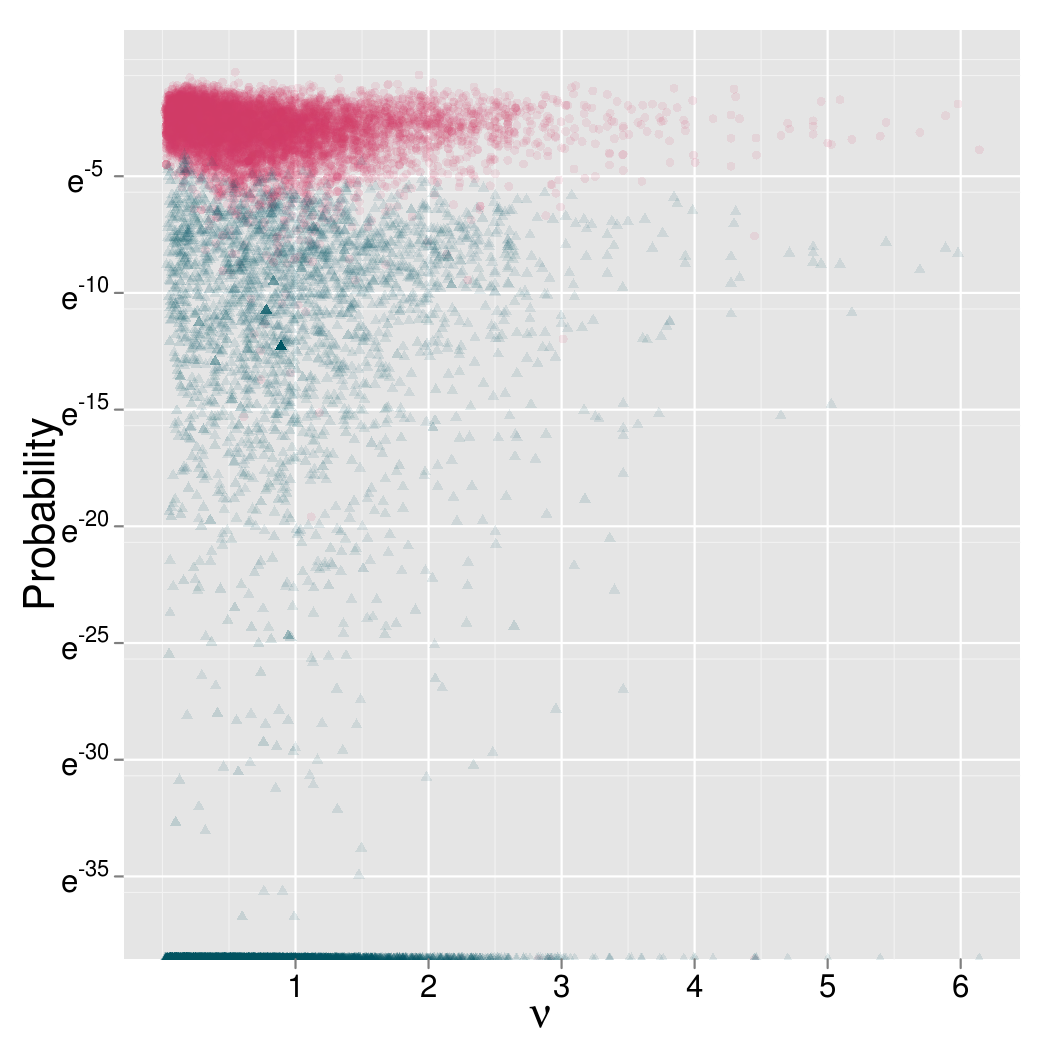
\includegraphics[width = 0.3\textwidth]{Athl-CloudTheta1}}
 \subfigure[]{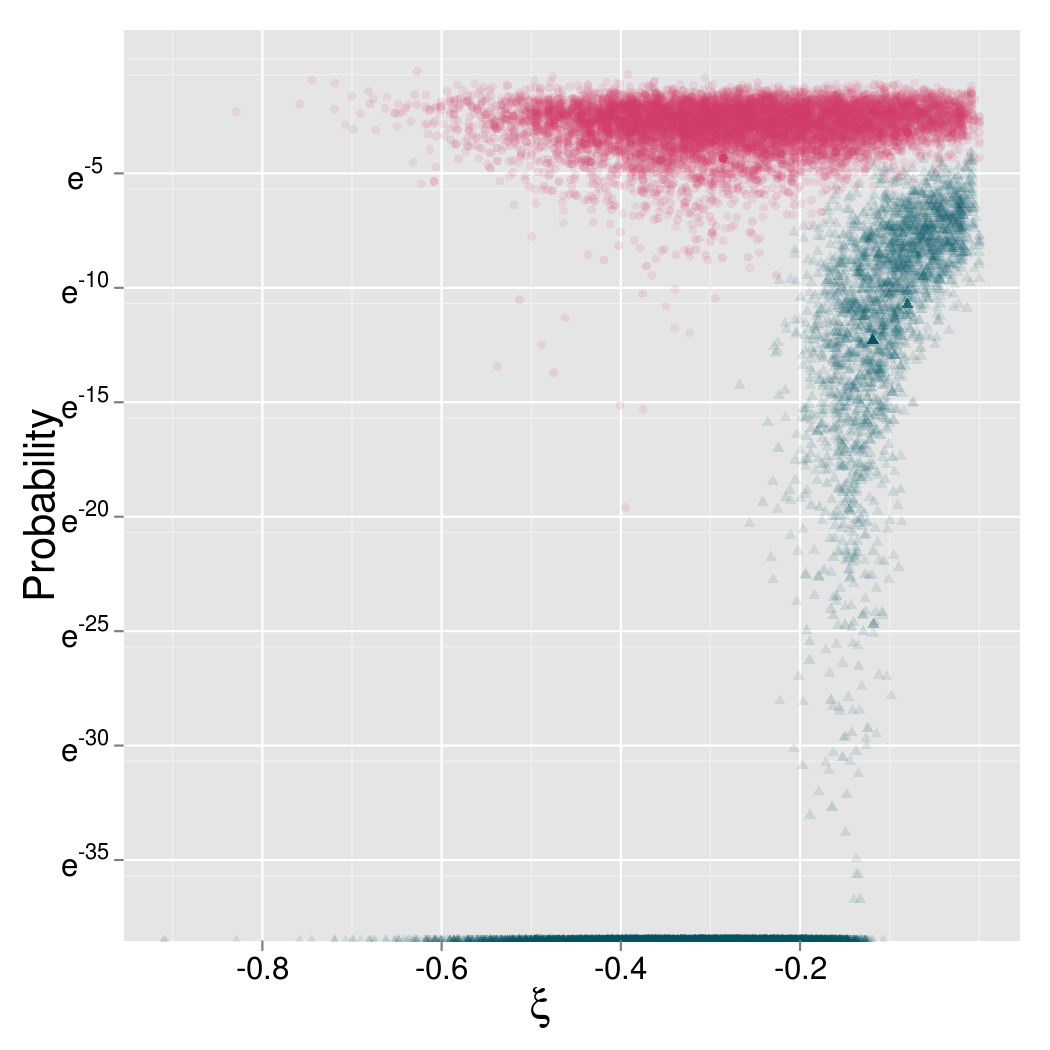
\includegraphics[width = 0.3\textwidth]{Athl-CloudTheta2}}
 \subfigure[]{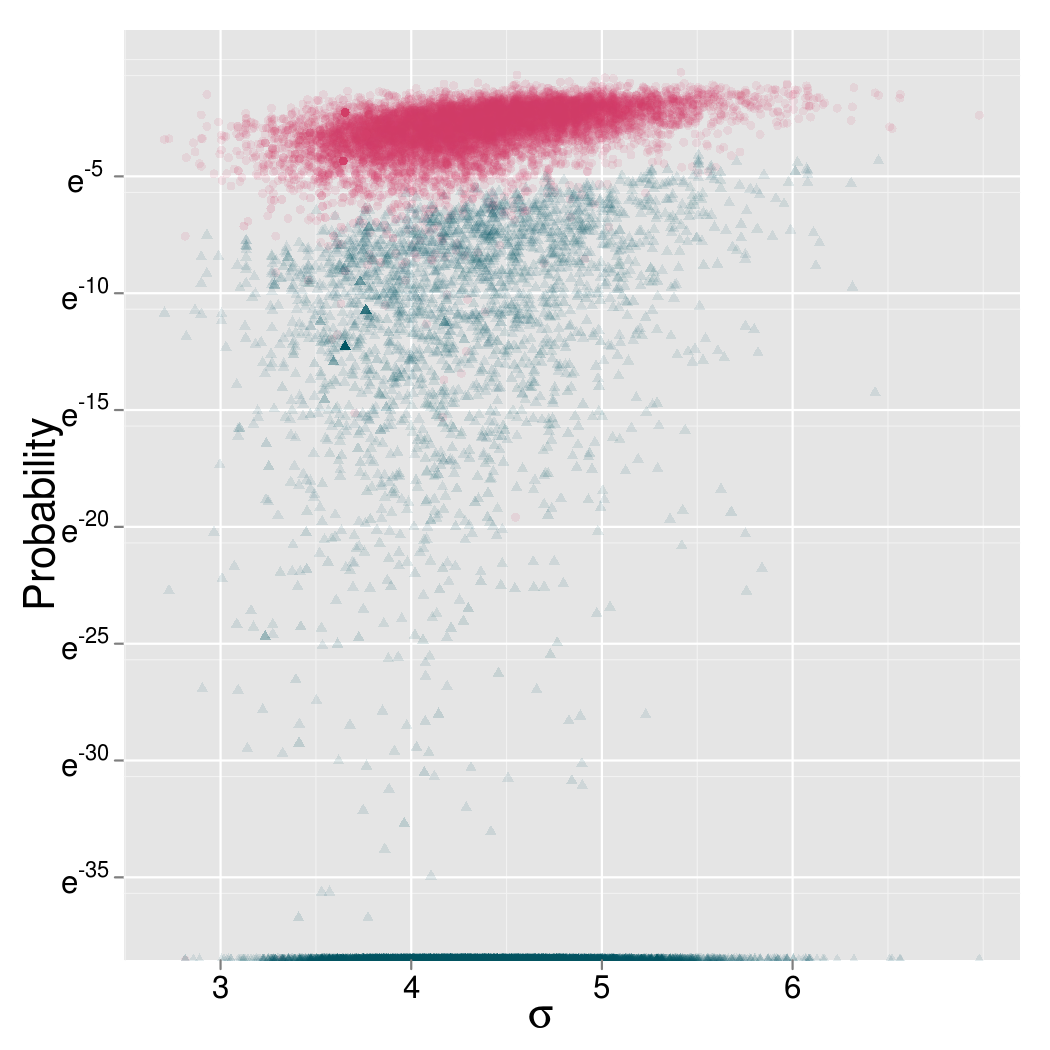
\includegraphics[width = 0.3\textwidth]{Athl-CloudTheta3}}
 \caption{\label{fig:athletics:perparameter} Athletics records: (first
row) posterior distribution of the
parameters approximated by the \SMCSQ algorithm, with $N_\theta =1,000$ and
$N_x = 250$. The kernel density
estimators, computed on $10$ independent runs, are overlaid on each plot. The
full
line represents the prior density function. (Second row) probability of
observing at year $1993$ a recorded time less than $486.11$ seconds (triangles,
lower cloud of points) and
less than $502.62$ seconds (circles, upper cloud of points) against the
components of $\theta$. Point sizes
and transparencies are proportional to the weights of the $\theta$-particles.}
\end{figure}

\bibliographystyle{apalike}
\bibliography{complete}
 
\end{document}
